\begin{block}{Algorithm Overview}
  \begin{figure}
  \centering
\begin{tikzpicture}[scale=1]
  \overview{(0cm,0cm)};
  \node[right=0.5cm of obs-edge] {\small 1. Solve bottlenecks};
  \node[right=0.5cm of cond-edge] {\objw{10cm}{\small 
  2a. Pseudoinverse \\
  2b. Composite likelihood
  }};
  \node[right=0.5cm of params-edge] {\obj{\small 
  3a. Renormalization \\
  3b. Convex optimization
  }};
\end{tikzpicture}
\end{figure}
\end{block}

\begin{block}{2. Exclusive views and bottlenecked graphs}
  \splitcolumn{%
    \begin{itemize}
      \item A variable $h_i \in S \subseteq \bh$ has an {\bf exclusive
        view} $x_v$ if
      \begin{itemize}
        \item there exists some observed variable $x_{v}$ which is
          conditionally independent of the others $S \backslash \{ h_i \}$
          given $h_i$.
        \item the conditional moments $\mOpp{v}{i} \eqdef \Pr(x_{v} \mid
          h_i)$ are full column rank $k$ and can be recovered.
      \end{itemize}
      \item {\bf Theorem:} Every bottlenecked bidependent set (think
        a clique) has exclusive views.
    \end{itemize}
  }{%
  \begin{figure}
    \centering
      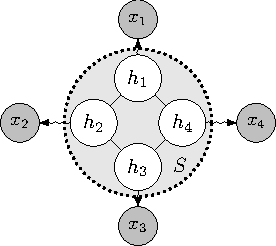
\includegraphics[width=0.95\textwidth,height=5cm,keepaspectratio]{figures/exclusive-views.pdf}
%      \caption{Exclusive views}
  \end{figure}
      
    \begin{itemize}
    \item Given {\em exclusive views}, $\Pr(x \given h)$,
      learning cliques is solving a linear equation.
      \begin{align*}
        M &= Z(\mOpp{1}{1}, \cdots, \mOpp{m}{m}) \\
        Z &= M(\mOppi{1}{1}, \cdots, \mOppi{m}{m}).
      \end{align*}
    \end{itemize}
  }
\end{block}
\begin{block}{2b. Composite likelihood for hidden marginals}
  \splitcolumn{

  \begin{figure}
    \centering
    \begin{tikzpicture}
      \point{stuff}{(2cm,2.5cm)};
      \drawhmm{(stuff)};
      \begin{pgfonlayer}{background}
      \draw[draw=black,fill=green!70,rounded corners,line width=1pt, dotted] 
                      ($(h1.west) + (180:0.3cm)$) -- 
                      ($(h1.north) + (90:0.3cm)$) -- 
                      ($(h2.north) + (90:0.3cm)$) -- 
                      ($(h2.east) + (0:0.3cm)$) -- 
                      ($(x2.east) + (0:0.3cm)$) -- 
                      ($(x2.south) + (-90:0.3cm)$) -- 
                      ($(x1.south) + (-90:0.3cm)$) -- 
                      ($(x1.west) + (180:0.3cm)$) -- 
                      cycle;
      \end{pgfonlayer}
    \end{tikzpicture}
  \end{figure}

  \begin{itemize}
    \item By fixing the conditional mom., the {\em composite
      likelihood} of a subset of variables is {\em convex}.
    \item Estimation with composite likelihoods is consistent
      (\cite{lindsay88composite}).
    \item Asymptotically, the composite likelihood estimator is {\em more
      efficient}.
  \end{itemize}

  }{%
  \begin{figure}
    \centering
    \includegraphics[width=\textwidth,height=6cm,keepaspectratio]{figures/asymp-k2d5-bordered.pdf}
    \caption{Comparison of the pseudoinverse and composite likelihood
    estimators on a HMM with $k=2$ hidden and $d=5$ observed values.
    }
  \end{figure}
  }
\end{block}

\begin{block}{3. Recovering parameters}
  \splitcolumn{%
  \begin{itemize}
    \item In directed models: CPTs can be recovered by normalization. 
    \item In undirected mdoels: $Z_{12}$ can be used to estimate {\em
      feature marginals} and can be solved by {\em convex optimization},
      similar to supervised learning.
    \item Can be used with pseudo-likelihoods to efficiently
      learn high-treewidth models.
  \end{itemize}
  }{% 
    \small

      \begin{align*}
        \Pr(h_2 \given h_1) &= \frac{\Pr(h_1, h_2)}{\sum_{h_2} \Pr(h_1, h_2)}.
        \end{align*}
\vfill
      \begin{align*}
          \sL(\theta) &= \theta^\top \mu_\sC + A(\theta) \\
          \mu_\sC &= 
              \sum_{\sC \in \sG} 
              \E_{(\bx,\bh) \sim \sD_\text{sup}}[\phi(\bx_\sC,\bh_\sC)] \\
                  &= \sum_{\bx_\sC, \bh_\sC} \underbrace{\mathmg{\Pr(\bx_\sC \given \bh_\sC)}}_{\textmg{cond. moments}} 
          \underbrace{\mathmb{\Pr(\bh_\sC)}}_{\textmb{hid. marg.}} \phi(\bx_\sC,\bh_\sC).
          \end{align*}
  }
\end{block}

\begin{block}{Conclusion}
  \splitcolumn{
  \begin{itemize}
    \item We provide an algorithm for {\bf any bottlenecked
      graphical model}, including {\em high treewidth} and {\em undirected graphical models}.
    \item Combining moment estimates with likelihood objectives
      provides a new perspective balancing efficiency and accuracy.
  \end{itemize}
  }{
  \centering
  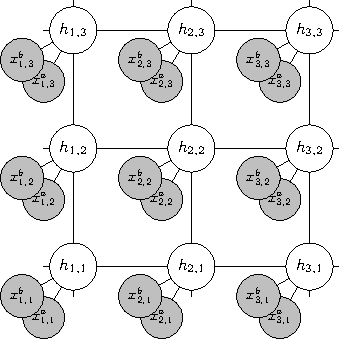
\includegraphics[width=\textwidth,height=5cm,keepaspectratio]{figures/mrf.pdf}
  }
\end{block}


